\documentclass[10pt]{beamer}

\newcommand{\lectnum}{L04}
\newcommand{\lecttitle}{Revisiting Regression}

\usepackage{amsmath, amssymb, graphicx}
\usepackage[]{algorithm2e}
\usepackage{pdfpages}
\usepackage[british]{babel}

\hypersetup{colorlinks,linkcolor=,urlcolor=blue}
\newenvironment{titledslide}[1]{\begin{frame}\frametitle{#1}}{\end{frame}}

\mode<presentation>{\setbeamercovered{transparent}}

\setbeamertemplate{sidebar right}{}
\setbeamertemplate{footline}{%
\hfill\usebeamertemplate***{navigation symbols}
\hspace{0.4cm}\lectnum: \insertframenumber{}/\inserttotalframenumber \hspace*{0.4cm}}

\author{James Cussens}

\title{COMS30035, Machine learning:\\ \vspace{5pt} \lecttitle}

\institute{School of Computer Science\\University of Bristol}

\begin{document}
%%%%%%%%%%%%%%%%%%%%%%%%%%%%%%%%%%%%%%%%%%%%%%%%%%%%%%%%%%%%%%%%%%%%%%

\begin{frame}
  \titlepage
\end{frame}

%%%%%%%%%%%%%%%%%%%%%%%%%%%%%%%%%%%%%%%%%%%%%%%%%%%%%%%%%%%%%%%%%%%%%%


%%%%%%%%%%%%%%%%%%%%%%%%%%%%%%%%%%%%%%%%%%%%%%%%%%%%%%%%%%%%%%%%%%%%%%
\begin{titledslide}{Acknowledgement}

  \begin{itemize}
  \item These slides are adapted from ones originally created by
    \href{https://www.dpag.ox.ac.uk/team/rui-ponte-costa}{Rui Ponte
      Costa} and Dima Damen and later edited by Edwin Simpson. 
  \end{itemize}
  
\end{titledslide}
%%%%%%%%%%%%%%%%%%%%%%%%%%%%%%%%%%%%%%%%%%%%%%%%%%%%%%%%%%%%%%%%%%%%%%
\begin{frame}[fragile]

  \frametitle{Textbooks}
  Chapter 3 of the Bishop book is directly relevant:
  \begin{itemize}
  \item Bishop, C. M., Pattern recognition and machine learning (2006). Available for free \href{https://www.microsoft.com/en-us/research/people/cmbishop/prml-book/}{here.}	\vspace{10pt}
  \item \textbf{Note:} this first part is a revision of should be
    covered in Data-driven Computer Science in your 2nd year.
\end{itemize}

\end{frame}
%%%%%%%%%%%%%%%%%%%%%%%%%%%%%%%%%%%%%%%%%%%%%%%%%%%%%%%%%%%%%%%%%%%%%%

\begin{frame}[fragile]
\frametitle{Agenda}
\begin{itemize}
		\item Linear regression
		\item Nonlinear regression		
		\item Probabilistic models
		\item Maximum likelihood estimation
\end{itemize}

\end{frame}
%%%%%%%%%%%%%%%%%%%%%%%%%%%%%%%%%%%%%%%%%%%%%%%%%%%%%%%%%%%%%%%%%%%%%%
\begin{frame}[fragile]
\frametitle{Revisiting regression}

\begin{itemize}
\item Goal: Finding a relationship between two variables \begin{small}(e.g. regress \emph{house value} against \emph{number of rooms})\end{small}
\vspace{12pt}
\item Model: Linear relationship between \emph{house value} and \emph{number of rooms}?
\end{itemize}
\vspace{6pt}
\centerline{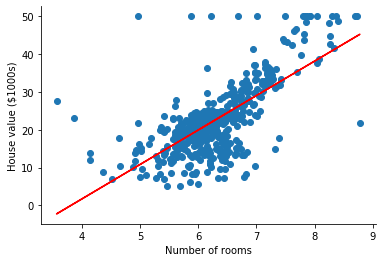
\includegraphics[scale=0.5]{../figures/boston_linear1.png}}
\end{frame}


%%%%%%%%%%%%%%%%%%%%%%%%%%%%%%%%%%%%%%%%%%%%%%%%%%%%%%%%%%%%%%%%%%%%%%
\begin{frame}[fragile]
  
\frametitle{Revisiting regression -- deterministic model}

\textbf{\textcolor{blue}{Data:}} a set of data points $D = \{ (x_1, y_1), (x_2, y_2), \cdots, (x_N, y_N) \}$ where $x_i$ is the number of rooms of house $i$ and $y_i$ the house value.
\vspace{6pt}

\textbf{\textcolor{blue}{Task:}} build a model that can predict the house value from the number of rooms
\vspace{6pt}

\uncover<2->{\textbf{\textcolor{red}{Model Type:}} parametric; assumes a polynomial relationship between house value and number of rooms}
\vspace{6pt}

\uncover<3->{\textbf{\textcolor{red}{Model Complexity:}} assume the relationship is linear $\text{house value} = a_0 + a_1 \times \text{rooms}$
\begin{equation}
y_i = a_0 + a_1 x_i
\end{equation}}
\vspace{6pt}

\uncover<4->{\textbf{\textcolor{red}{Model Parameters:}} model has two parameters $a_0$ and $a_1$ which should be estimated.

\begin{itemize}
\item $a_0$ is the y-intercept
\item $a_1$ is the slope of the line
\end{itemize}}

\end{frame}
%%%%%%%%%%%%%%%%%%%%%%%%%%%%%%%%%%%%%%%%%%%%%%%%%%%%%%%%%%%%%%%%%%%%%%
\begin{frame}[fragile]
  
\frametitle{Revisiting linear regression -- fitting}
\begin{itemize}
\item Find $a$ and $b$ which minimises 
\begin{equation}
R(a,b) = \sum_{i=1}^N {(y_i - (a + bx_i))^2}
\nonumber
\end{equation}
\item This is the \textcolor{blue}{sum of residuals}.
\item A method which gives a closed form solution is to minimise the sum of squared vertical offsets of the points from the line, \textbf{\textcolor{blue}{Method of Least-Squares}}
\end{itemize}
\vspace{6pt}

\end{frame}
%%%%%%%%%%%%%%%%%%%%%%%%%%%%%%%%%%%%%%%%%%%%%%%%%%%%%%%%%%%%%%%%%%%%%%

\begin{frame}[fragile]

  \frametitle{Least Squares Solution - \textcolor{blue}{matrix form}}
  \begin{itemize}
  \item To find a solution to the parameters $\theta = \{a_0, a_1\}$
    solve least squares problem which \textcolor{blue}{in matrix form},
    means to find \textcolor{blue}{$\textbf{a}_{LS}$}
  \end{itemize}
  
  \begin{align}
    \uncover<2->{& \textcolor{blue}{\textbf{a}_{LS}} = (\textbf{X}^T \textbf{X})^{-1} \  \textbf{X}^T \  \textbf{y}}
  \end{align}

\vspace{4pt}
\uncover<3->{\begin{itemize}
  \item Here $X_{i,j}$ is the value of the $j$th feature in the $i$th
    datapoint (where we add a fake feature which is always 1 to handle
    the intercept), and $y_i$ is the value of the \emph{response} in the
    $i$th datapoint.
  \item Matrix formulation also allows least squares method to be extended to \textbf{\textcolor{blue}{polynomial fitting}}
  \item For a polynomial of degree $p+1$ we use \begin{tiny}(note: $p>1$ gives nonlinear regression)\end{tiny}
    \begin{equation}
      y_i = a_0 + a_1 x_i + a_2 x_i^2 + \cdots + a_{p} \ x_{i}^{p} \nonumber
    \end{equation}
  \end{itemize}}

\end{frame}
%%%%%%%%%%%%%%%%%%%%%%%%%%%%%%%%%%%%%%%%%%%%%%%%%%%%%%%%%%%%%%%%%%%%%%


\begin{frame}[fragile]
\frametitle{Least Squares Solution}
\begin{example}
Find the best least squares fit by a linear function to the data using $p=1$

\begin{center}
\begin{tabular}{c|c|c|c|c}
x &-1 &0 &1 &2\\ \hline
y &0 &1 &3 &9
\end{tabular}
\end{center}
\end{example}

\uncover<2->{$\textbf{y} = \begin{bmatrix} 0\\ 1\\ 3\\ 9 \end{bmatrix}$} \hspace{6pt} \uncover<3->{$\textbf{X} = \begin{bmatrix} 1 &-1\\ 1&0\\ 1 &1\\ 1 &2 \end{bmatrix}$}
\hspace{6pt} \uncover<4->{$\textbf{X}^T \textbf{X} = \begin{bmatrix} 1 &1 &1 &1\\ -1 &0 &1 &2 \end{bmatrix} \begin{bmatrix} 1 &-1\\ 1&0\\ 1 &1\\ 1 &2 \end{bmatrix} = \begin{bmatrix} 4 &2\\ 2 &6\end{bmatrix}$}\\
\vspace{6pt}

\uncover<5->{$\textbf{a}_{LS} = (\textbf{X}^T \textbf{X})^{-1} \textbf{X}^T \textbf{y}$} \uncover<6->{$= \frac{1}{20} \begin{bmatrix} 6 &-2\\ -2 &4 \end{bmatrix}$} \uncover<7->{$\begin{bmatrix} 1 &1 &1 &1\\ -1 &0 &1 &2 \end{bmatrix}$} \uncover<8->{$\begin{bmatrix} 0\\ 1\\ 3\\ 9 \end{bmatrix}$} \uncover<9->{$= \begin{bmatrix} 1.8\\ 2.9 \end{bmatrix}$}

\uncover<10->{$y = 1.8 + 2.9 x$}
\end{frame}




\begin{frame}[fragile]
\frametitle{Regression with probabilistic models}

\begin{small}\textbf{Probabilistic models are a core part of ML}, as they allow us to also capture the uncertainty the model has about the data, which is critical for real world applications. For simplicity, lets drop $a_0$ from the previous model and add a random variable $\epsilon$ that captures the uncertainty \end{small}
\begin{equation*}
\text{house price} = a_1 \times \text{number of rooms} + \epsilon
\end{equation*}


\uncover<2->{We can assume, for example, that $\epsilon$ is given by $\mathcal{N}(\mu=0, \sigma^2)$ which gives the likelihood
\begin{align*}
p(\textbf{y}|\textbf{X},\theta) &= \prod\limits_{i=1}^N{p(\text{price}_i | \text{rooms}_i, \theta)} = \prod\limits_{i=1}^N {\frac{1}{\sqrt{2 \pi} \sigma} e^{-\frac{1}{2}\frac{(\text{price}_i - a_1\text{rooms}_i)^2}{\sigma^2}}}
\end{align*}}

%\begin{equation*}
%p(\epsilon) = \frac{1}{\sqrt{2 \pi} \sigma} e^{-\frac{\epsilon^2}{2 \sigma^2}}
%\end{equation*}}

\uncover<3->{\small This model has \textcolor{red}{two} parameters: the slope $a_1$ and variance $\sigma$ \footnote{\tiny Note that here $\mu = a_0$ which, for simplicity, we assume to be zero.}
\vspace{0pt}

\centerline{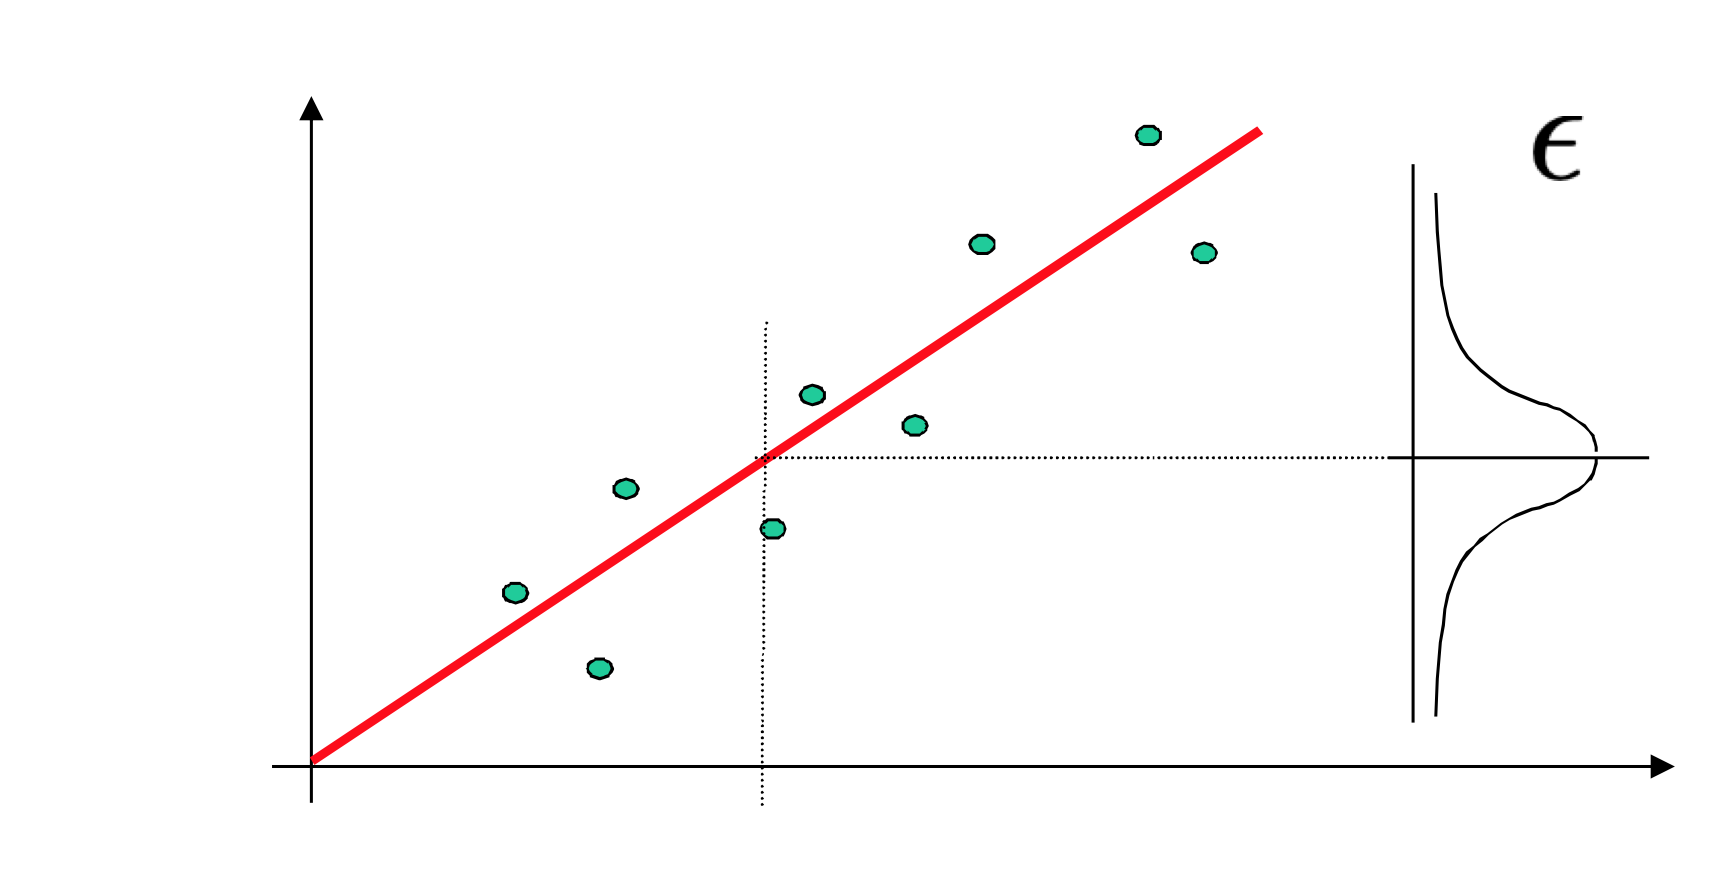
\includegraphics[scale=0.15]{../figures/probabilistic_line.png}}}

\end{frame}





\begin{frame}[fragile]
\frametitle{Maximum Likelihood Estimation}

\begin{itemize}
\item Similar to building deterministic models, probabilistic model parameters need to be tuned/trained
\item \textbf{\textcolor{blue}{Maximum-likelihood estimation (MLE)}} is a method of estimating the parameters of a probabilistic model.
\vspace{8pt}
\uncover<2->{\item Assume \textcolor{blue}{$\boldsymbol{\theta}$}  is a vector of all parameters of the probabilistic model. (e.g. $\boldsymbol{\theta} = \{a_1, \sigma\}$).
\item \textbf{\textcolor{blue}{MLE}} is an extremum
  estimator\footnote{\begin{tiny} ``Extremum estimators are a wide class of estimators for parametric models that are calculated through maximization (or minimization) of a certain objective function, which depends on the data.'' wikipedia.org\end{tiny}} obtained by maximising an objective function of $\boldsymbol{\theta}$}
\end{itemize}

\end{frame}

\begin{frame}[fragile]
\frametitle{Maximum Likelihood Estimation}

\begin{definition}
Assume $f(\theta)$ is an objective function to be optimised (e.g. maximised), the \textcolor{blue}{$arg\,max$} corresponds to the value of $\theta$ that attains the maximum value of the objective function $f$

\vspace{8pt}
\uncover<2->{\begin{equation*}
\hat{\theta} = arg\,max_{\theta} \, f(\theta)
\end{equation*}}
\end{definition}

\begin{itemize}
%\uncover<3->{\item \textbf{\textcolor{red}{Note:}} this is different than maximising the function (i.e. finding the maximum value [$max \, f(\theta)$])}
\uncover<3->{\item  Tuning the parameter is then equal to finding the maximum argument $arg\,max$}

\end{itemize}

\end{frame}


\begin{frame}[fragile]
\frametitle{Maximum Likelihood Estimation - General}

\begin{itemize}
\item Maximum Likelihood Estimation (MLE) is a common method for solving such problems
\begin{align*}
\theta_{MLE} &= arg\,max_\theta \, p(D|\theta)\\
 &= arg\,max_\theta \, \ln p(D|\theta)\\
 &= arg\,min_\theta \, -\ln p(D|\theta)
\end{align*}
\vspace*{-6pt}
\uncover<2->{\begin{block}{MLE Recipe}
\begin{enumerate}
\vspace{6pt}
\uncover<3->{\item Determine $\theta$, $D$ and expression for likelihood $p(D|\theta)$}
\vspace{6pt}
\uncover<4->{\item Take the natural logarithm of the likelihood}
\vspace{6pt}
\uncover<5->{\item Take the derivative of $\ln p(D|\theta)$ w.r.t. $\theta$. If $\theta$ is a multi-dimensional vector, take partial derivatives}
\vspace{6pt}
\uncover<6->{\item Set derivative(s) to 0 and solve for $\theta$}
\end{enumerate}
\end{block}}
\end{itemize}

\end{frame}

%\begin{frame}[fragile]
%\frametitle{MLE: 1. Define likelihood}
%
%Given a set of N data points - $x_i$ is length and $y_i$ is weight in our \textit{fishy} example
%\begin{equation*}
%D = \{ (x_1, y_1), (x_2, y_2), \cdots, (x_N, y_N) \}
%\end{equation*}
%
%\begin{itemize}
%\uncover<2->{\item The probabilistic approach would:
%\begin{itemize}
%\item derive expression for conditional probability of observing data $D$ given parameters $\boldsymbol{\theta} = \{b, \sigma\}$
%\begin{equation*}
%p(D | \theta)
%\end{equation*}}
%\vspace{6pt}
%
%%\uncover<3->{\item using observed data, find the parameter value that maximises the conditional probability (or likelihood)
%%\begin{equation*}
%%a_{ML} = arg\,max_a p(D|a)
%%\end{equation*}
%\end{itemize}
%\end{itemize}
%
%\end{frame}

%\begin{frame}[fragile]
%\frametitle{MLE: 1. Define likelihood}
%
%Given a set of N data points
%\begin{equation*}
%D = \{ (x_1, y_1), (x_2, y_2), \cdots, (x_N, y_N) \}
%\end{equation*}
%
%\uncover<2->{Assume that observations are independent - a common assumption often referred to as \textbf{i.i.d. independent and identically distributed} - then :
%\begin{equation*}
%p(D|\theta) = \prod\limits_{i=1}^N {p(y_i | x_i, \theta)}
%\end{equation*}}
%
%\uncover<3->{Given $y_i = b \, x_i + \epsilon$, and $\epsilon$ is $\mathcal{N}(0, \sigma^2)$, then
%\begin{equation*}
%p(y_i | x_i, \theta) \sim \mathcal{N} (b x_i, \sigma^2)
%\end{equation*}}
%
%\uncover<4->{For a large sample:
%\begin{itemize}
%\item The average of $y_i$ value will be $b \, x_i$}
%\uncover<5->{\item The `spread' or variance will be the same as for $\epsilon$, defined by $\sigma^2$}
%\end{itemize}
%
%\end{frame}
%
%\begin{frame}[fragile]
%\frametitle{MLE: 1. Define likelihood}
%
%The conditional probability (for all data) is thus formulated as
%\begin{align*}
%p(D|\theta) &= \prod\limits_{i=1}^N{p(y_i | x_i, \theta)} \\
% &= \prod\limits_{i=1}^N {\frac{1}{\sqrt{2 \pi} \sigma} e^{-\frac{1}{2}\frac{(y_i - bx_i)^2}{\sigma^2}}}
%\end{align*}
%
%\end{frame}
%
%
%
%
%
%
%\begin{frame}[fragile]
%\frametitle{MLE: 2. Take natural logarithm}
%
%We will focus on parameter $b$ for the next steps,
%\vspace*{-10pt}
%
%{\small
%\begin{align*}
%b_{ML} &= arg\,max_b \, p(D|\theta)\\
%\uncover<2->{&= arg\,max_b \prod\limits_{i=1}^N {\frac{1}{\sqrt{2 \pi} \sigma} e^{-\frac{1}{2} \frac{(y_i - bx_i)^2}{\sigma^2}}}}\\
%\uncover<3->{&= arg\,max_b \ln{\Bigl(\prod\limits_{i=1}^N {\frac{1}{\sqrt{2 \pi} \sigma} e^{-\frac{1}{2} \frac{(y_i - bx_i)^2}{\sigma^2}}}\Bigr)} \qquad \textcolor{orange}{\text{(use $\ln$ trick)}}}\\
% \uncover<4->{&= arg\,max_b \sum\limits_{i=1}^N \ln{\Bigl(\frac{1}{\sqrt{2 \pi} \sigma} e^{-\frac{1}{2} \frac{(y_i - bx_i)^2}{\sigma^2}}\Bigr)} \qquad \textcolor{orange}{\text{($\ln$ prop. 1)}}}\\
% \uncover<5->{&= arg\,max_b \sum\limits_{i=1}^N \ln{\frac{1}{\sqrt{2 \pi} \sigma} -{\frac{(y_i - bx_i)^2}{2\sigma^2}}} \qquad \textcolor{orange}{\text{($\ln$ prop. 2)}}}\\
% \uncover<6->{&=arg\,max_b \sum\limits_{i=1}^N {-\frac{1}{2\sigma^2}(y_i - b x_i)^2} \qquad \textcolor{orange}{\text{(discard no-b terms $\ln{\frac{1}{\sqrt{2 \pi} \sigma}}$)}}}\\
% \uncover<7->{&=arg\,min_b \sum\limits_{i=1}^N {\frac{1}{2\sigma^2}(y_i - bx_i)^2}\qquad \textcolor{orange}{\text{(switch to minimisation form.)}}}\\
%\end{align*}}
%
%\end{frame}
%
%\begin{frame}[fragile]
%\frametitle{Data Modelling - Deterministic vs Probabilistic}
%
%\begin{itemize}
%\item Deterministic Least Squares [Lecture 3]:
%\begin{equation*}
%b_{LS} = arg\,min_b \, R(b,a=0) = arg\,min_b \sum_i (y_i - b\, x_i)^2
%\end{equation*}
%\item Probabilistic Maximum Likelihood:
%\begin{equation*}
%b_{ML} = arg\,min_b \sum_i  \textcolor{blue}{\frac{1}{2\sigma^2}}(y_i - b\, x_i)^2
%\end{equation*}
%
%\uncover<2->{\item \textcolor{blue}{probabilistic model explicit considers uncertainty, $\sigma^2$.}}
%%\uncover<3->{\item \textbf{\textcolor{blue}{Note:}} ML answer here assumes uncertainty is normally distributed}
%\end{itemize}
%
%\end{frame}
%
%\begin{frame}[fragile]
%\frametitle{MLE: 3. Take derivatives and 4. Find solution}
%
%To simplify the calculations here we assume $\sigma = 1$,
%\begin{equation*}
%b_{ML} = arg\,min_b \sum_i \frac{1}{2}(y_i - b\, x_i)^2
%\end{equation*}
%
%\uncover<2->{To find the minimum, calculate the derivative
%\begin{equation*}
%\frac{d}{db}{\sum_i \frac{1}{2}(y_i - b x_i)^2} = -\sum_i x_i (y_i - b x_i)
%\end{equation*}}
%
%\uncover<3->{and equate it to zero
%\begin{align*}
%&-\sum_i x_i (y_i - b_{ML} x_i) = 0\\
%&\sum_i x_i y_i - b_{ML} \sum_i x_i^2 = 0\\
%&b_{ML} = \frac{\sum_i {y_i x_i}}{\sum_i x_i^2}
%\end{align*}}
%
%\end{frame}

%\begin{frame}[fragile]
%\frametitle{MLE: example}
%
%\begin{block}{Example: normal distribution (parameter $a_1$)}
%\begin{enumerate}
%\vspace{6pt}
%\uncover<2->{\item Determine $\theta$, $D$ and expression for likelihood $p(D|\theta)$}
%\uncover<3->{\\$
%p(D|{a_1}) = \prod\limits_{i=1}^N {\frac{1}{\sqrt{2 \pi} \sigma} e^{-\frac{1}{2}\frac{(y_i - {a_1}x_i)^2}{\sigma^2}}}$}
%\vspace{6pt}
%\uncover<4->{\item Take the natural logarithm of the likelihood}
%\uncover<5->{\\$
%{a_1}_{ML} = arg\,min_{a_1} \sum_i \frac{1}{2\sigma^2}(y_i - {a_1}\, x_i)^2$
%}
%\vspace{6pt}
%\uncover<6->{\item Take the derivative of $\ln p(D|\theta)$ w.r.t. $\theta$. If $\theta$ is a multi-dimensional vector, take partial derivatives \footnote{For simplicity we set $\sigma = 1$}}
%\uncover<7->{\\$
%\frac{d}{d{a_1}}{\sum_i \frac{1}{2}(y_i - {a_1} x_i)^2} = -\sum_i x_i (y_i - {a_1} x_i)
%$
%}
%\vspace{6pt}
%\uncover<7->{\item Set derivative(s) to 0 and solve for $b$}
%\uncover<8->{\\$
%{a_1}_{ML} = \frac{\sum_i {y_i x_i}}{\sum_i x_i^2}
%$
%}
%\end{enumerate}
%\end{block}
%
%\end{frame}
%%%%%%%%%%%%%%%%%%%%%%%%%%%%%%%%%%%%%%%%%%%%%%%%%%%%%%%%%%%%%%%%%%%%%%
\begin{titledslide}{Least Squares and MLE for Linear Regression}

  \begin{itemize}
  \item In the case of standard linear regression one can prove that
    the parameters which minimise the squared error are also the MLE
    parameters.
  \item Note that in general the MLE recipe just given will only find
    local maxima of the likelihood (so not necessarily the MLE).
  \item But in the special case of linear regression it does find the MLE.
  \end{itemize}
  
\end{titledslide}

%%%%%%%%%%%%%%%%%%%%%%%%%%%%%%%%%%%%%%%%%%%%%%%%%%%%%%%%%%%%%%%%%%%%%%
\begin{frame}[fragile]
\frametitle{Data Modelling - Deterministic vs Probabilistic}

\begin{itemize}
\item \textbf{\textcolor{blue}{Probabilistic Models}} can tell us \textcolor{red}{more}
\uncover<2->{\item We could use the same MLE recipe to find \textcolor{red}{$\sigma_{ML}$}. This would tell us how uncertain our model is about the data $D$.}
\uncover<3->{\item For example: if we apply this method to two datasets ($D_1$ and $D_2$) what would the parameters $\theta = \{{a_1},\sigma\}$ be?}
\end{itemize}
\uncover<4->{\centerline{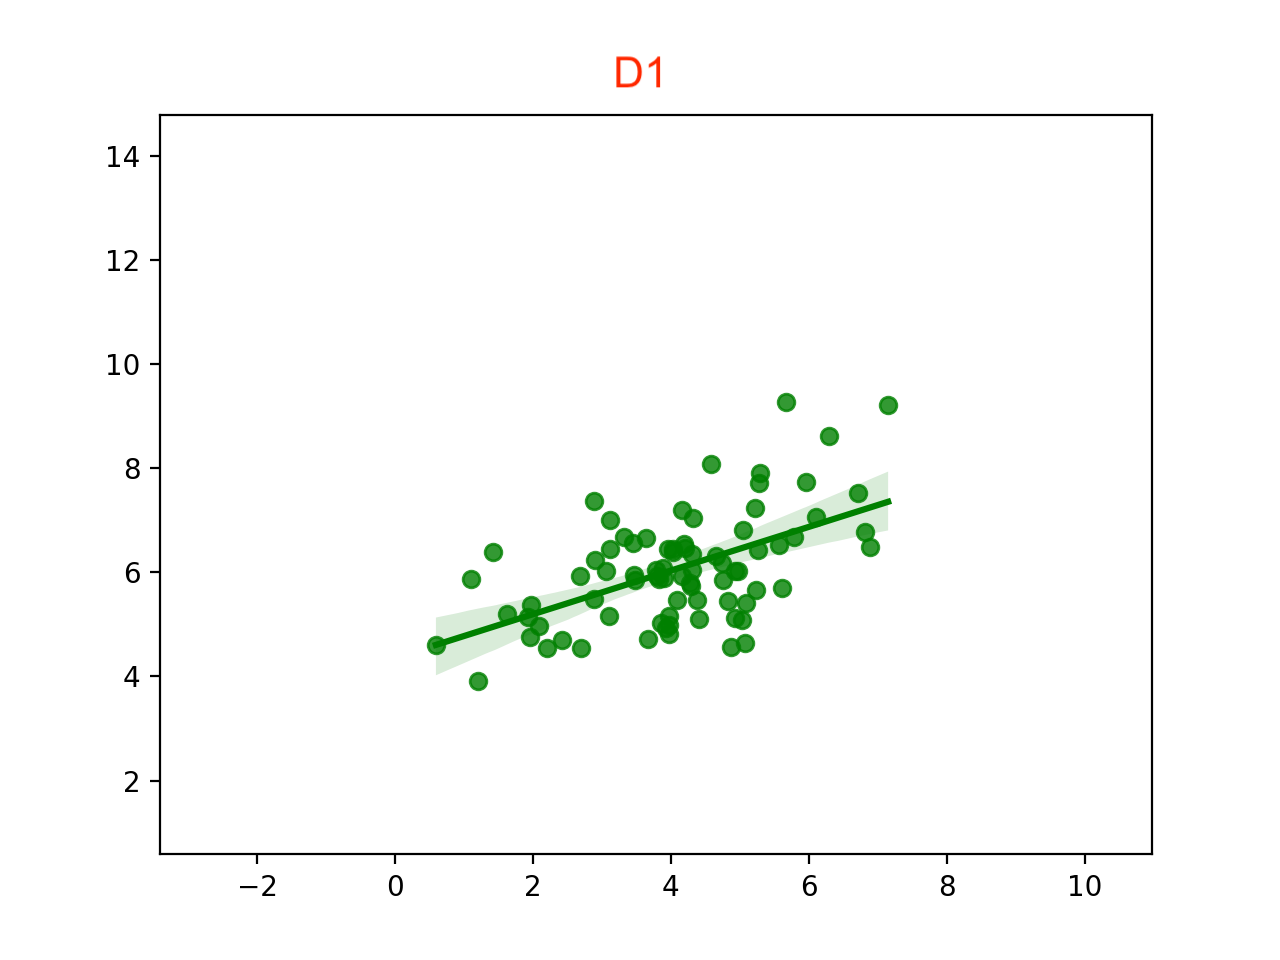
\includegraphics[scale=0.35]{../figures/low_var.png}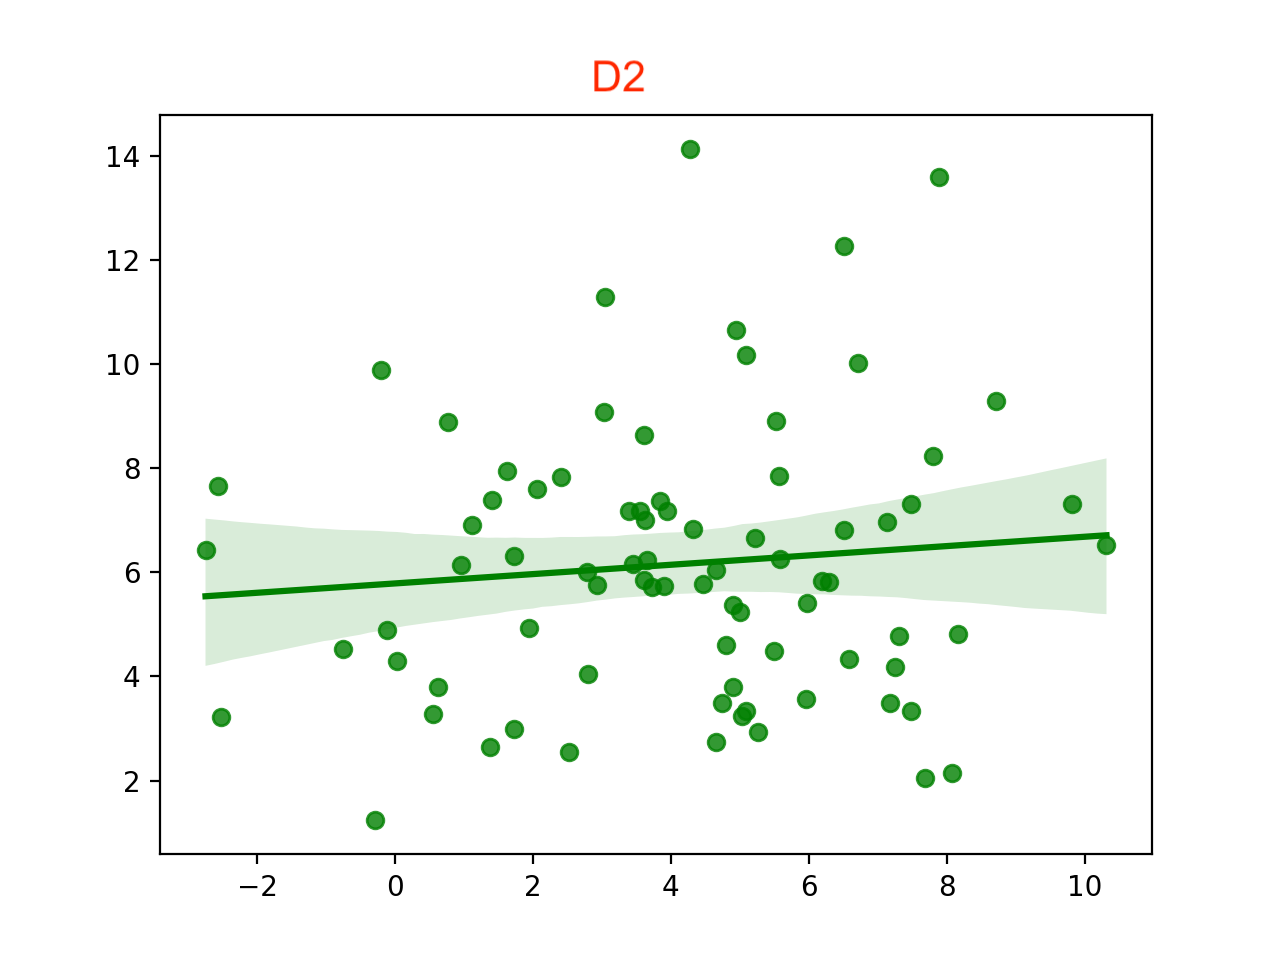
\includegraphics[scale=0.35]{../figures/high_var.png}}}

\uncover<5->{\centerline{${a_1}_{ML}^{D_1} > {a_1}_{ML}^{D_2} \:$ \small{[slope]} and \textcolor{red}{$\: \sigma_{ML}^{D_1} < \sigma_{ML}^{D_2}$ \small{[uncertainty\footnote{The uncertainty ($\sigma$) is represented by the light green bar in the plots. Test it yourself.}]}}}}

\end{frame}

\begin{frame}[fragile]
\frametitle{Quiz time!}
\centerline{
\includegraphics[scale=0.3]{../figures/BB.png}\vspace{10pt}}
\begin{center}\begin{Large} Go to Blackboard unit page $\gg$ Quizzes $\gg$ Week 1,  Revisiting Regression \end{Large}\end{center}\vspace{10pt}
\centerline{[Should take you less than 5 minutes]}
\end{frame}

\end{document}
